\section{Framework Grundlagen}

\begin{itemize}
	\item OO Klassen die Zusammenarbeiten
	\item Verfügt über Erweiterungspunkte / Hooks
	\item Steuert den Kontrollfluss (im Gegensatz zu einer Library); ``main()'' lebt im Framework \\
		``Hollywood Principle: Don't call us, we call you''
	\item Stellt nützliche Klassen zur Verfügung
\end{itemize}

\textbf{Application Frameworks}

Dienen zur Wiederverwendung von Infrastruktur für ähnliche Applikationen in einem gemeinsamen Kontext.

Die Entwicklung ist oft Evolutionär und wird von einigen konkreten Applikationen getrieben, von denen Gemeinsamkeiten ins Framework übertragen werden.

\textbf{Micro Frameworks}

Einige Pattern stellen Micro Frameworks mit Erweiterungspunkten, Hooks und der Steuerung des Kontrollflusses dar.

\begin{itemize}
	\item Template Methods - Die Template Method in der AbstractClass steuert den Kontrollfluss; Die PrimitiveOperations bilden Hook Methods
	\item Strategy - ...
	\item Command Processor

	\begin{figure}[H]
		\centering
		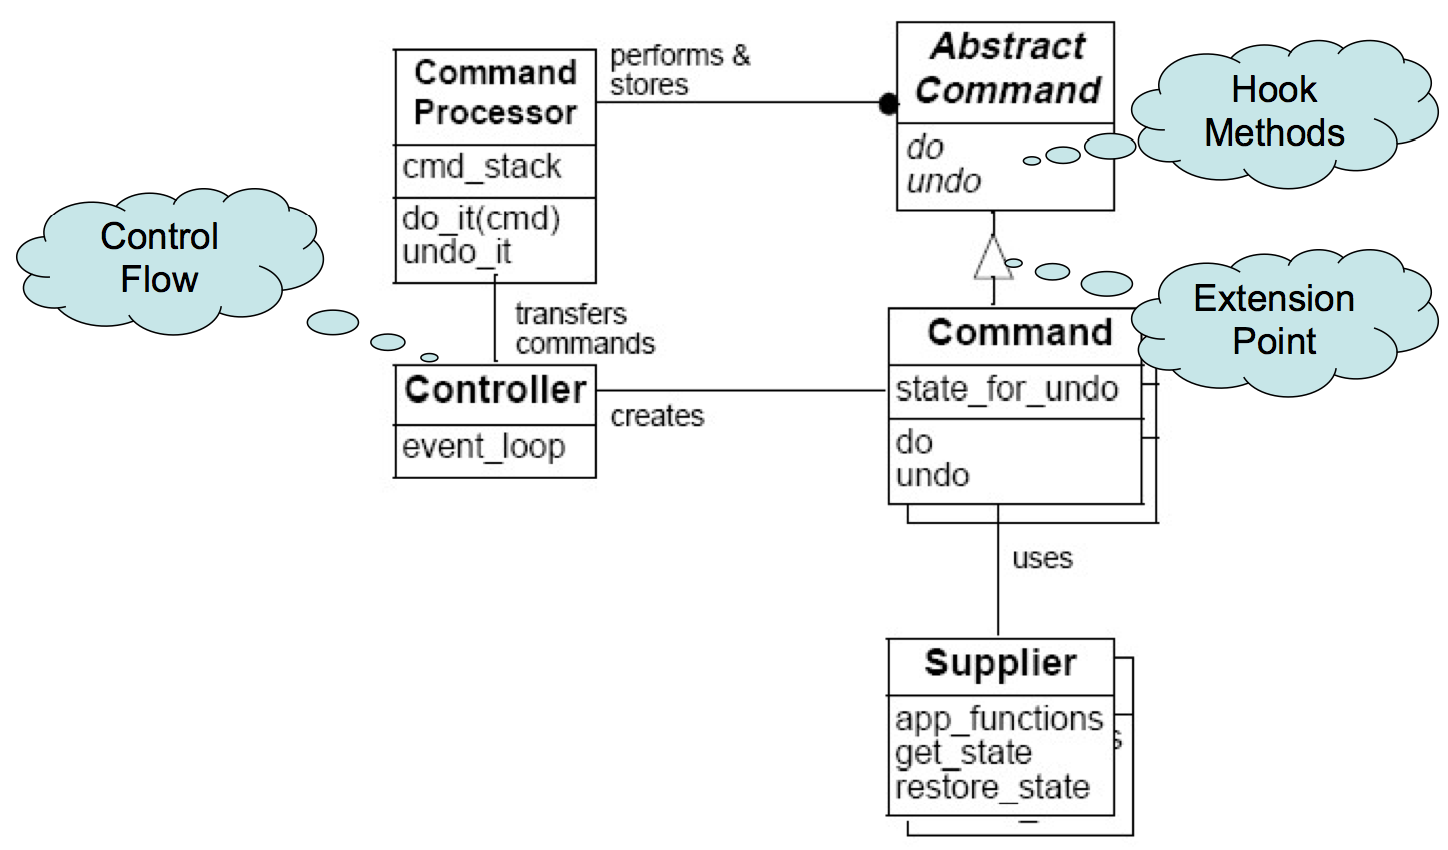
\includegraphics[width=0.9\textwidth]{content/frameworks/commandprocessormicroframework.png}
		\caption{Command Processor als Microframework}
	\end{figure}
\end{itemize}